\documentclass{standalone}
\usepackage{pgfplots}
\usetikzlibrary{shapes.geometric, intersections}
\pgfplotsset{compat=1.7}

\begin{document}
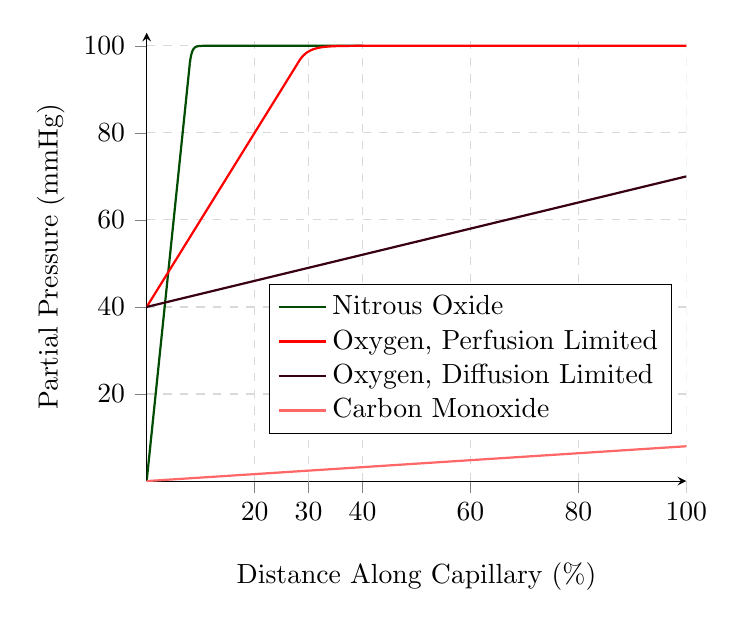
\begin{tikzpicture}

    \begin{axis}[
        axis x line=middle,
        axis y line=middle,
        grid = major,
        grid style={dashed, gray!30},
        xmin=0,     % start the diagram at this x-coordinate
        xmax= 100,    % end   the diagram at this x-coordinate
        ymin= 0,     % start the diagram at this y-coordinate
        ymax= 103,   % end   the diagram at this y-coordinate
	 ylabel near ticks,
	xlabel near ticks,
	extra x ticks={30},
        xlabel=Distance Along Capillary (\%),
        ylabel=Partial Pressure (mmHg),
        tick align=outside,
        enlargelimits=false,
legend style={at={(0.6,0.44)},anchor=north},
legend cell align={left}]

	\addplot[domain=0:8, green!30!black, thick,samples=500] {12*x)};
	\addlegendentry{Nitrous Oxide}

	\addplot[domain=0:28, red, thick,samples=500] {40+2*x)};
	\addlegendentry{Oxygen, Perfusion Limited}

	\addplot[domain=0:100, purple!30!black, thick,samples=500] {40+0.3*x)};
	\addlegendentry{Oxygen, Diffusion Limited}

	\addplot[domain=0:100, red!60!white, thick,samples=500] {0.08*x)};
	\addlegendentry{Carbon Monoxide}


	\addplot[domain=8:40, green!30!black, thick,samples=500] {4*(1-exp(-2.5*(x-8)))+96)};
	\addplot[domain=28:100, red, thick,samples=500] {4*(1-exp(-0.56*(x-28)))+96)};




\end{axis}

\end{tikzpicture} 
\end{document}